\newpage

\section{Q2}


\begin{figure}[htbp]
    \centering
    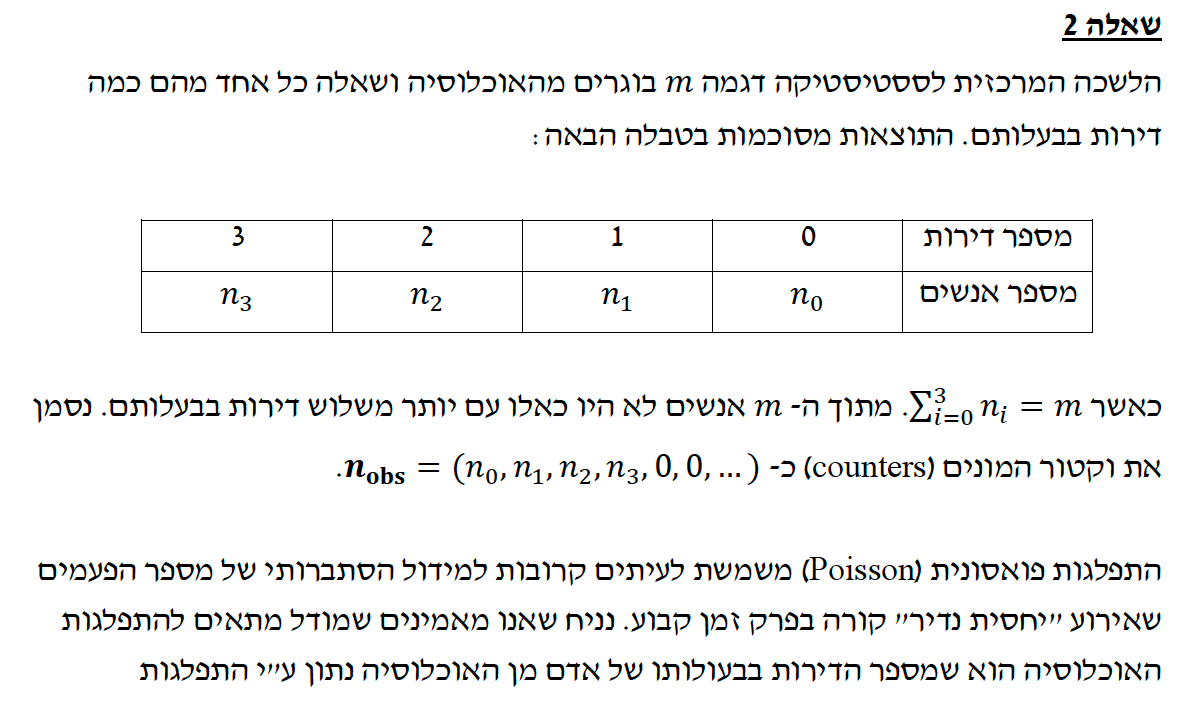
\includegraphics[width=0.48\linewidth]{images/q21.png}
    \caption{q2}\label{fig:q21}
\end{figure}

\begin{figure}[htbp]
    \centering
    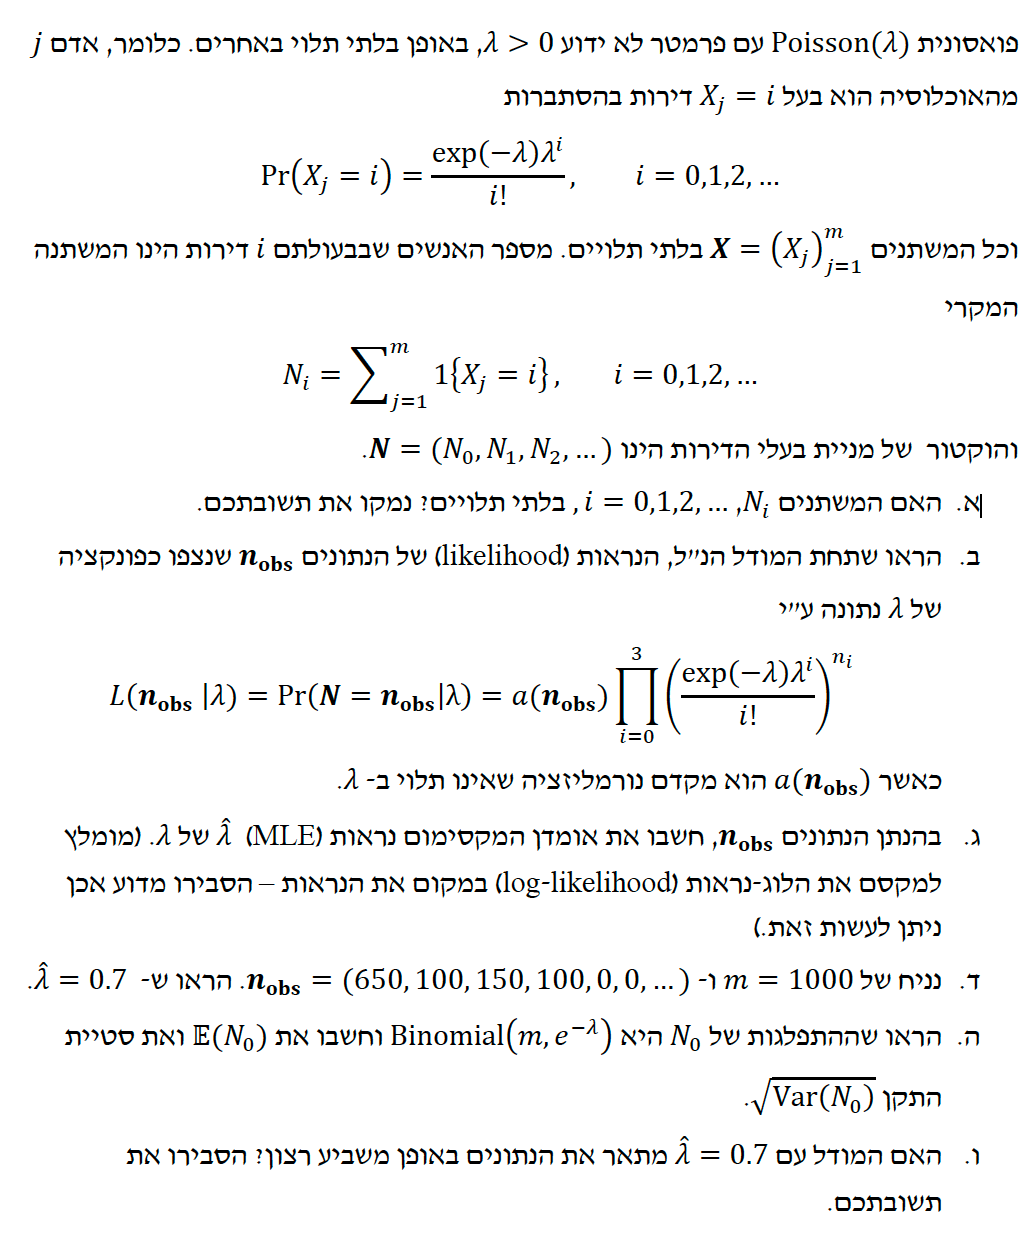
\includegraphics[width=0.48\linewidth]{images/q22.png}
    \caption{q2}\label{fig:q22}
\end{figure}


The Central Bureau of Statistics sampled graduates 
from the population and asked each of them how many
apartments they owned. The following results follow:

\begin{table}[htbp]
    \centering
    \begin{tabular}{|l|l|l|l|l|}
    \hline
    apartments Number & 0 & 1 & 2 & 3 \\ \hline
    People Number & $n_0$ & $n_1$ & $n_2$ & $n_3$ \\ \hline
    \end{tabular}
    \caption{}\label{table:example_2x5}
\end{table}

such that $\sum_{i=0}^{3} n_i = m $ from the m people, no one has more than 3 apartments.
denote the counters vector as $n_obs=(n_0,n_1,n_2,n_3,0,0,\dots)$

$Poisson(\lambda)$ with unknown parameter $\lambda > 0$ independently of others.
and all the variables $X=(X_j)^m_j=1$ are independent.

The number of people who own $i$ apartments is the random variable:
$N_i=\sum_{j=1}^{m} 1\left\{X_j=i\right\}, i=0,1,2,\dots$
and the vector of counting apartments owners is $N=(N_0,N_1,N_2,\dots)$

\subsection{Q2.1}
Does the variables $N_i , i=0,1,2,\dots$ statistically independent?
Justify your answer. - answer NO they are not.

\textbf{Solution:} \\
Two variables $X$ and $Y$ are statistically independent if and only if
% the occurrence of one does not affect the probability of occurrence of 
% the other, which can be mathematically defined as:
\[P(X \cap Y) = P(X)P(Y)\]

therefore for $N_i$ it means for any $i \neq j$ the following holds:
\[P(N_i \cap N_j) = P(N_i)P(N_j)\]

Given constraint $\sum_{i=0}^{3} n_i = m$, where $m$ is the fixed,
it makes dependency for $N_i$ variables because if say $N_0=1$ then
if effects the probability of others $N_i, i\neq 0 $ because 
we know 1 member has 0 apartments. 

remember for Poisson distribution $P(X=k)=\frac{\lambda^k e^{-\lambda}}{k!}$

for example consider this case for $m=3$ and $\lambda=1$
denote : \\
 $P(X=1)=\frac{1^1 e^{-1}}{1!}=e^{-1}=0.368$
 and \\
 
 $P(X=2)=\frac{1^2 e^{-1}}{2!}=\frac{e^{-1}}{2}=0.184$
\[ 
    P(N_1=1)= \binom{3}{1} P(X=1)^1(1-P(X=1))^{3-1}= \binom{3}{1}  (0.368)  (1-0.368)^2 = 0.44
\]
\[ 
    P(N_2=1)= \binom{3}{1} P(X=2)^1(1-P(X=2))^{3-1} =\binom{3}{1} (0.184)  (1-0.184)^2 =  0.36
\]
\[
    P(N_1=1)P(N_2=1) = 0.44 \cdot 0.36 = 0.15
\]

Now consider the case where 1 person with 1 apartment, and 1 person with 2 apartments, and 1 person
with 0 apartments(no apartments).

\[
    P(N_1 = 1 \cap N_2 = 1) = 3 \times P(X=1)\times P(X=2) \times P(no apartments)   
\]

the number 3 is for the permutations. P(X=1) and P(X=2) with $\lambda = 1$ already calculated

\[
    P(N_1 = 1 \cap N_2 = 1) = 3 \times e^{-1} \times \frac{ e^{-1}}{2} \times (1- e^{-1} - \frac{ e^{-1}}{2}) = 0.09 \neq 0.15 =  P(N_1=1)P(N_2=1)
\]

by showing this contradicting example, we can understand that the variables are not independent



% q2.2

\subsection{Q2.2}
Show that over this model, the likelihood of $n_obs$ observerd as a function of $\lambda$
is given by
$ L(n_obs|\lambda)=Pr(N=n_obs|\lambda)=a(n_obs)\prod_{i=0}^{3}\left(\frac{\exp(-\lambda)\lambda^i}{i!} \right)^{n_i} $

where $a(n_obs)$ is a normalization coefficient that does not depend on $\lambda$

\indent \textbf{Solution:} \\

From Q2.1 we conclude that the variables $N_i$ are not independent, therefore The
likelihood is not directly the product of the probabilities.
Because number of apartments owners is fixed(m), and distributed among 4 categories, 
and not $\infty$ categories, summing the probability of only 4 categories will not equal to 1, 
also this case fit into the Multinomial Distribution
\[
    \sum_{i=0}^{\infty}P(X=i) = 1 \neq \sum_{i=0}^{3}P(X=i)
\]

for Multinomial distribution $P(X_1=x_1,\dots,X_k=x_k)=\frac{n!}{x_1!\dots x_k!} p_1^{x_1}\dots p_k^{x_k}$
therfore if follows that 
\[
L(n_obs|\lambda) = \frac{m!}{n_0!n_1!n_2!n_3!} \prod_{i=0}^{3} \left( \frac{e^{-\lambda}\lambda^i}{i!} \right)^{n_i} 
\]

it is clear that $a(n_obs)=\frac{m!}{n_0!n_1!n_2!n_3!}$ and that it is not depends on $\lambda$ 

this equality $ L(n_obs|\lambda)=Pr(N=n_obs|\lambda) $ follows because $L(n_obs|\lambda)$ determining the likely 
to specific data , and $Pr(N=n_obs|\lambda)$ calculates the probability for specific data therefore the equality holds.

\subsection{Q2.3}
Given $n_obs$ calculates the MLE $hat{\lambda}$ of $\lambda$. (it is recommended to maximize the 
log-likelihood instead of the likelihood - \textbf{Explain why this can indeed be done} )

\indent \textbf{Solution:} \\

From Q2.2
\[
    L(n_obs|\lambda) = \frac{m!}{n_0!n_1!n_2!n_3!} \prod_{i=0}^{3} \left( \frac{e^{-\lambda}\lambda^i}{i!} \right)^{n_i}     
\]

The log-likelihood as recommended from the question 
\[ 
    \ln(L(n_obs|\lambda)) = \ln(a(n_obs)) + \sum_{i=0}^{3} n_i \left(\ln(e^{-\lambda}) + \ln(\lambda^i) - \ln(i!) \right)
\]
\textbf{This can indeed be done} because $a>b$ so $\log(a) > \log(b)$
note that $\ln(e^{-\lambda}) = -\lambda $
\[ 
    \ln(L(n_obs|\lambda)) = \ln(a(n_obs)) + \sum_{i=0}^{3} n_i \left( -\lambda + i\ln(\lambda) - \ln(i!) \right)
\]

note that $ln(a(n_obs))$ and $-ln(i!)$ are constants with respect to $\lambda$ therefore their derivation is zero.
lets derive and set equal to zero:
\[
    \frac{d}{d\lambda} \ln(L(n_obs|\lambda)) = \sum_{i=0}^{3} n_i (-1+\frac{i}{\lambda}) = 0
\]

\[
    \sum_{i=0}^{3} n_i (-1+\frac{i}{\lambda}) = 0    
\]

\[
    \sum_{i=0}^{3}(-n_i)  \sum_{i=0}^{3}(\frac{n_i i}{\lambda}) = 0    
\]

\[
    - \sum_{i=0}^{3}(n_i)  \frac{1}{\lambda}\sum_{i=0}^{3}(n_i i) = 0    
\]

\[
    \frac{1}{\lambda}\sum_{i=0}^{3}(n_i i) = \sum_{i=0}^{3}(n_i)    
\]

\[
    \lambda = \frac{\sum_{i=0}^{3}(n_i i)}{\sum_{i=0}^{3}(n_i)    }  
\]

$i \in {0,1,2,3}$ then for i=0 $n_0 \cdot 0 = 0 $ therefore

\[
   \hat{\lambda} = \frac{n_1 + 2 n_2  + 3 n_3  }{n_0 + n_1 + n_2 + n_3}  
\]

\subsection{Q2.4}
Assume that $m = 1000$ and $n_obs = (650,100,150,100,0,0,\dots)$ show that $\hat{\lambda} = 0.7 $

\indent \textbf{Solution:} \\
\[
   \hat{\lambda} = \frac{100 + 2\cdot 150  + 3\cdot 100  }{650 + 100 + 150 + 100} = 0.7  
\]

\subsection{Q2.5}
show that the distribution of $N_0$ is $Binomial(m,e^{-\lambda})$ and calculate $E(N_0)$
and the variance $\sqrt{Var(N_0)}$

\indent \textbf{Solution:} \\
We know that $N_0$ is a Poisson distribution that a person has 0 apartments $P(X=0) = \frac{e^{-\lambda} \lambda^0}{0!} = e^{-\lambda}$ 
since in the scenario are m people and each of them has $e^{-\lambda}$ of owning 0 apartments out of m
it follows a fit to Binomial distribution $Binomial(m,e^{-\lambda})$
Then the expectation follows from the Binomial distribution 
\[
    E(N_0)=m\cdot e^{-\lambda}  
\]

and the variance also follows from the Binomial distribution as

\[
    Var(N_0) = m \cdot e^{-\lambda} \cdot (1-e^{\lambda})    
\]

the standard deviation is 

\[
    sqrt{Var(N_0)} = sqrt{m \cdot e^{-\lambda} \cdot (1-e^{\lambda}) } 
\]

these just follows from the poisson and binomial distribution.




\subsection{Q2.6}

\indent \textbf{Solution:} \\




